% !TEX root = main.tex

%%%%%%%%%%%%%%%%%%%%%%%%%%%%%%%%%%%%%%%%%%%%%%%%%%%%%%
\section{実験目的}
%%%%%%%%%%%%%%%%%%%%%%%%%%%%%%%%%%%%%%%%%%%%%%%%%%%%%%
制御系設計には
\begin{itemize}
  \item 運動方程式や回路方程式などから制御対象のモデル(微分方程式,伝達関数など)を導出する
  \item モデルに含まれるパラメータを実験により決定する(パラメータ同定)
  \item 制御対象の出力(制御量)を所望の値にするような制御対象の入力(操作量)を決めるためにコントローラの設計を行う
\end{itemize}
というモデリングの作業と
\begin{itemize}
  \item 制御対象の出力(制御量)を所望の値にするような制御対象の入力(操作量)を決めるためにコントローラの設計を行う
\end{itemize}
というコントローラ設計の作業が含まれる.
本実験では,平面上に回転するアームの角度制御を例として,制御系設計の一連の流れを習得することを
目的としている.

\section{ロボットアーム実験装置の概要と制御目的}

\subsection{ロボットアーム実験装置}

図 2.1 に示すように,ロボットアーム実験装置はアームが水平にして DC モータにより回転するようになっている.
DC モータを駆動させるためにパソコン上で計算された指令電圧は,I/O ボード "Q8-USB" により D/A 変換され,
アンプを介して DC モータに入力される.
さらに,アームの角度はシャフトに取り付けてあるポテンショメータによって角度として検出され,
I/O ボード "Q8-USB" により A/D 変換されて後,パソコンに取り込まれている.

\subsection{アクチュエータと D/A 変換}

コンピュータから出力される指令電圧はデジタル値であるため,D/A 変換によってアナログ値に変換される
(図 2.2 に示す).アナログ周期ごとに一定値のアクションに変換してからアンプに加える必要がある.
指令電圧の I/O ボード "Q8-USB" による D/A 変換には,16 ビットが使われており,
分解能は \(0.30518 [V] = (\pm 10 - (-10))/2^{16} \)[V] の刻み幅である.

\begin{figure}[h]
  \centering
  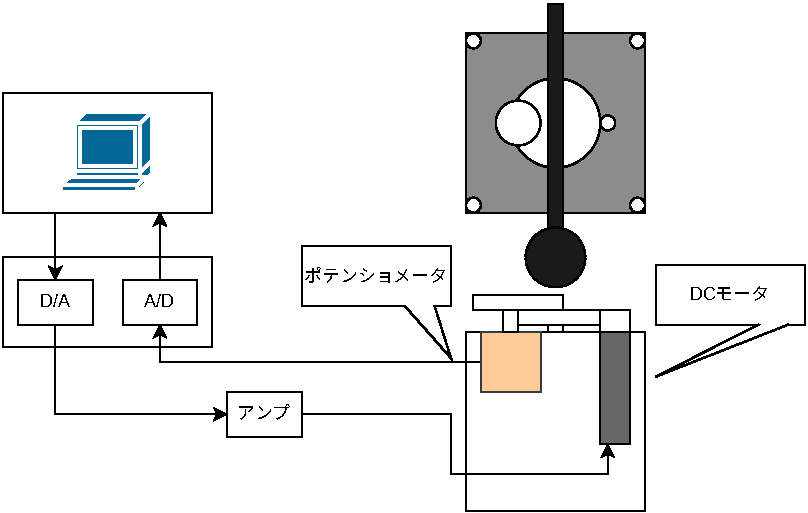
\includegraphics[scale=0.4]{sozai/1.pdf}
  \caption{ロボットアーム実験装置}
\end{figure}

\begin{figure}[h]
  \centering
  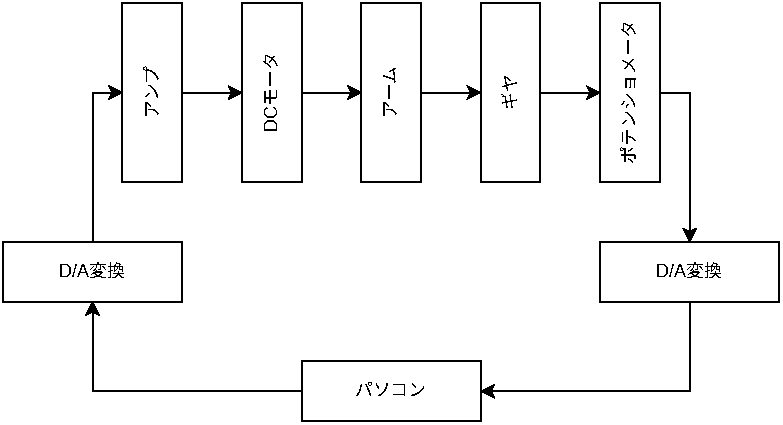
\includegraphics[scale=0.65]{sozai/2.pdf}
  \caption{制御対象のブロック線図}
\end{figure}

\subsection{センサと A/D 変換}

本実験装置では,ロボットアームの角度を検出するためのセンサにポテンショメータが用いられている.
ポテンショメータは可変抵抗であり角度に比例した電圧(アナログ量)\(V_s \)[V] を返す.
センサの出力電圧とロボットアームの角度との関係は,1 [V] あたり \(-35\) [deg] であり,
\(-175 \sim 175\) [deg] の角度を検出可能である.

コンピュータでこのセンサ電圧 \(V_s(t) \)[V] を利用するには,
A/D 変換によってアナログ量をサンプリング周期 [s] でディジタル量に変換する必要がある.
A/D 変換では,\(V_s(kh) \)[V] のように \(V_s(t)\) を横軸(時間軸)方向に離散化する標本化の作業と,
\(V_s(kh)\) を縦軸方向に離散化する量子化の作業を行う.
本実験装置の I/O ボード "Q8-USB" 上の A/D 変換部はレンジ:\(\pm 5 \)[V] または \(\pm 10 \)[V],
分解能:16 ビットである.本実験では,レンジを \(\pm 5 \)[V] に設定しているため,
約 \(0.15259 [mV] = (\pm 5 - (-5))/2^{16} \)[V] の刻み幅(量子化サイズ)で量子化することになる.

\subsection{制御目的と P 制御}

本実験では,ロボットアームの回転角度を所望の角度ですばやく止める角度制御を考える.
角度制御を実現するために考えられる最も単純な方法は,
\begin{itemize}
  \item 目標角 \( \theta_{\text{ref}}(t) \) と回転角 \( \theta(t) \) の差(偏差と呼ぶ)を計算
  \item その差が正(負)に大きければ正(負)の大きな電圧 \(v(t)\) を加える
  \item 正(負)に小さければ正(負)の小さな電圧 \(v(t)\) を加える
\end{itemize}
という方法である.このように偏差 \(e(t) = \theta_{\text{ref}}(t) - \theta(t)\) 
に比例した電圧 \(v(t)\) を加えるような制御方法をP制御(比例制御)という.また,
\begin{equation}
  v(t) = k_{\mathrm{P}} e(t) \quad \Longleftrightarrow \quad v(s) = k_{\mathrm{P}} e(s)
\end{equation}
という形式のコントローラをPコントローラと呼ぶ.


\begin{figure}[h]
  \centering
  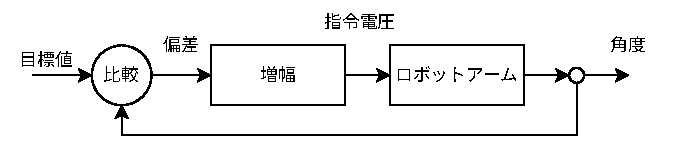
\includegraphics[scale=1]{sozai/3.pdf}
  \caption{P制御}
\end{figure}

\begin{figure}[h]
  \centering
  \includegraphics[scale=1]{sozai/group03/ad_da/ad_da_conv-crop.pdf}
  \caption{P制御}
\end{figure}

\subsection{PI 制御}
P 制御では様々な要因でステップ状の目標値に対する定常偏差が生じることがある.
この定常偏差を零にするためには,コントローラに積分動作 \( k_I /s \) を含ませればよく,

\begin{equation}
  v(t) = k_{\mathrm{P}} e(t) + k_I \int_{0}^{t} e(\tau) d\tau \quad \Longleftrightarrow \quad v(s) = \left( k_{\mathrm{P}} + \frac{k_I}{s} \right)e(s)
\end{equation}

という形式のコントローラを PI コントローラと呼ぶ.


\section{実験 1 -- A/D, D/A 変換の動作確認と P, PI 制御 --}

\subsection{実験装置のセッティング}
ロボットアーム実験装置が図~3.1 のように結線されていることを確認する.


\begin{figure}[h]
  \centering
  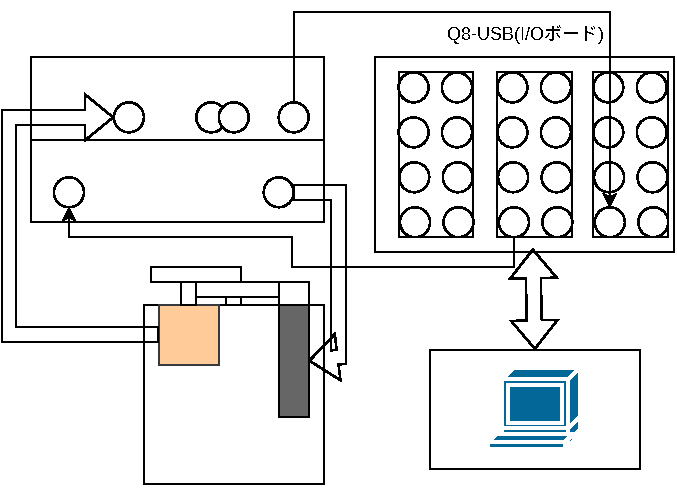
\includegraphics[scale=0.8]{sozai/4.pdf}
  \caption{ロボットアーム実験装置の結線}
\end{figure}

\subsection{D/A 変換とアクチュエータの動作確認}
\begin{enumerate}
  \item D/A 変換の動作確認をするために図~3.2 の Simulink モデル ``da\_conv.slx'' を作成する.
        保存場所は D:\#student\_5S\#group01\#da (``01'' は班の番号であり,
        2 班なら ``01'' を ``02'' に読み替え)とする.Simulink モデルをビルドし,
        エラーがないことを確認した後,
        \begin{lstlisting}
  >> print -s -dpdf da_conv.pdf    ※結果確認 (3.7 節) で使うので必須
  >> print -s -dbitmap da_conv.bmp ※Word でレポートを書く場合
  \end{lstlisting}
        と入力して Simulink モデル ``da\_conv.slx'' の pdf ファイル ``da\_conv.pdf'' を生成する.
        さらに,生成した pdf ファイルの余分な空白を取り除くため,``da\_conv.pdf'' をデスクトップ上の
        ``bcpdfcrop-multi.bat'' にドラッグする.その結果,``da\_conv-crop.pdf'' が生成される.
        
        なお,QuaRC により利用できる Simulink ブロック HIL Initialize や HIL Write Analog については
        補足 1.1,パラメータ設定については補足 1.2, 1.3, ビルドと実行の方法については補足 1.4 を参照すること
        (別紙「補足事項:QuaRC の使用方法」).
  \item Simulink モデル “da\_conv.slx” のブロック Manual Switch を “Constant” 側にする.Simulink モデルの実行を開始すると,DC モータに一定の電圧が加わり,アームが一定速度で回転することを確認せよ.
  \item テスタを Universal Power Module の “OUT” と “GND” に接続する.図 3.2 の Constant ブロックを表 3.1 のように設定したときのテスタの測定値およびアームの動作を観測し,表 3.1 を完成せよ.
  \item Universal Power Module の “To Load” に接続されているケーブルの DC モータ側を取り外し,オシロスコープを Universal Power Module の “OUT” と “GND” に接続する.(オシロスコープの電圧レンジは 5 [V/DIV],時間レンジは 2 [msec/DIV] に設定する.\\
        \quad Simulink モデル “da\_conv.slx” のブロック Manual Switch を “Sine Wave” 側にする.ブロック “Sine Wave” の周波数を “pi/0.008” [rad/s],振幅を “5”,“10”,“15” と設定したとき,D/A 変換された電圧をオシロスコープで観測し,デジタルカメラで撮影せよ(付録 A.1 の 図 A.1 を参照).
\end{enumerate}

\subsubsection{実験結果}
以下に結果を示す.

\begin{figure}[h]
  \centering
  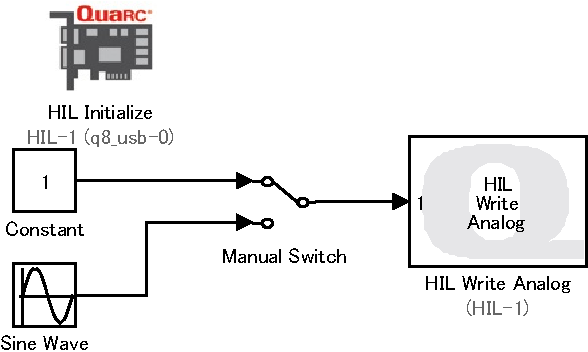
\includegraphics[scale=1]{sozai/da_conv-crop.pdf}
  \caption{da\_conv}
\end{figure}

\newpage

\begin{table}[h]
  \centering
  \caption{D/A 変換の動作確認とアームの回転方向}
  \begin{tabular}{|c|c|c|}
    \hline
    ブロック Constantの設定値 [V] & テスタによる測定値 [V] & 回転方向 (時計回り,反時計回り,静止) \\ \hline
    -5                            & -5                     & cww                                   \\ \hline
    -2.5                          & -2.494                 & cww                                   \\ \hline
    -1                            & -0.994                 & csww                                  \\ \hline
    -0.5                          & -0.495                 & cww                                   \\ \hline
    0                             & \(4.7×10^{-3}\)        & 静止                                  \\ \hline
    0.5                           & 0.504                  & cw                                    \\ \hline
    1                             & 1.003                  & cw                                    \\ \hline
    2.5                           & 2.502                  & cw                                    \\ \hline
    5                             & 5                      & cw                                    \\ \hline
  \end{tabular}
\end{table}

\begin{figure}[h]
  \centering
  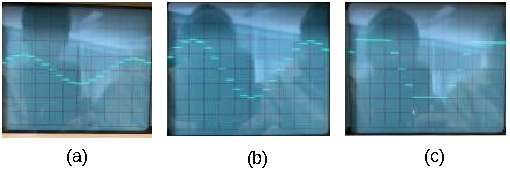
\includegraphics[scale=2]{sozai/5.pdf}
  \caption{オシロスコープ a=5,b=10,c=15}
\end{figure}

\subsubsection{実験考察}
da\_convにより設定値[v]がマイナスのとき反時計回り(ccw),プラスのときに時計回り(cw)となることが
表3.1よりわかる.また,出力値をテスターで計測したところほぼ設定値と同程度の電圧が測定できた.
これによりconstantの値をそのまま出力していることがわかる.

次にオシロスコープでは,振幅を5,10,15と変化させ観測したが,すべて16個の線により表されていた.
これは以下の式よりわかる.

周波数 \( f \) を \( \omega = \frac{\pi}{0.008} \, \text{[rad/s]} \) の場合に求めるには,
角周波数 \( \omega \) と周波数 \( f \) の関係を使用する.
\begin{equation}
  \omega = 2\pi f
\end{equation}
この式からより

\begin{equation}
  f = \frac{\omega}{2\pi}
\end{equation}

となり,角周波数 \( \omega = \frac{\pi}{0.008} \) の場合,

\begin{equation}
  f = \frac{\frac{\pi}{0.008}}{2\pi} = \frac{1}{2 \times 0.008} = \frac{1}{0.016} = 62.5 \, \text{[Hz]}
\end{equation}

つまり,角周波数が \( \frac{\pi}{0.008} \, \text{[rad/s]} \) の場合,
周波数 \( f \) は \( 62.5 \, \text{[Hz]} \) となる.
よって
\begin{equation}
  T = \frac{1}{f}
\end{equation}
\begin{equation}
  T = \frac{1}{62.5} = 0.016 \, \text{[s]}
\end{equation}

したがって,周期 \( T \) は \( 0.016 \, \text{[s]} \) となる.そのため,16個の線により表された.


\subsection{A/D変換とセンサの動作確認}
\begin{enumerate}
  \item A/D変換の動作確認をする図3.3のSimulinkモデル“ad\_conv.slx”を作成する.保存場所は D:\#student\_5S\#group01\#ad とする.ビルドしてエラーがないことを確認した後,printコマンドにて“ad\_conv.pdf”という名前のpdfファイルを生成し,デスクトップ上の“bcpdfcrop-multi.bat”により余白を取り除く.
  \item テスタをUniversal Power Moduleの“S1”と“GND”に接続し,アームを±45度に動かす(目測で良い).そのときのDisplay値とテスタの値を観測し,表3.2を完成せよ.
  \item 表3.2の結果から,センサ電圧1[V]あたりの角度変位を求めよ(符号に注意).
        \begin{equation}
          \text{センサ電圧 1 [V] あたりの角度変位} = {\large\textbf{     }} \, \text{[deg]} = {\large\textbf{     }} \, \text{[rad]}
        \end{equation}
  \item アームを1回転させたとき,センサ電圧の範囲をテスタにより測定せよ.
        \begin{equation}
          \text{センサ電圧:最小値} = {\large\textbf{     }} \, \text{[V]} , \quad \text{最大値} = {\large\textbf{     }} \, \text{[V]}
        \end{equation}
\end{enumerate}


\subsubsection{実験結果}
以下に結果を示す.

\begin{figure}[h]
  \centering
  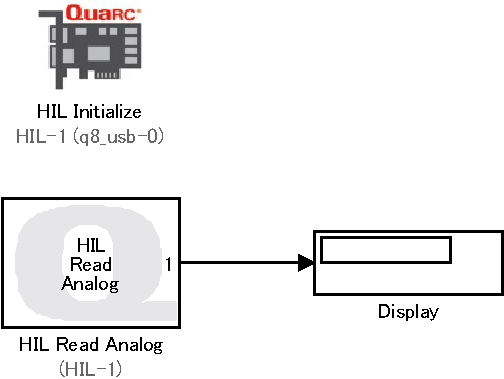
\includegraphics[scale=1]{sozai/ad_conv-crop.pdf}
  \caption{ad\_conv}
\end{figure}

\newpage

\begin{table}[h]
  \centering
  \caption{A/D変換の動作確認(角度:反時計回りが正)}
  \begin{tabular}{|c|c|c|}
    \hline
    アームの回転角度 [deg] & テスタによる測定値 [V]  & Displayによる測定値 [V] \\ \hline
    45                     & {\large\textbf{1.030}}  & {\large\textbf{1.031}}  \\ \hline
    0                      & --                      & --                      \\ \hline
    -45                    & {\large\textbf{-1.520}} & {\large\textbf{-1.521}} \\ \hline
  \end{tabular}
\end{table}

\begin{equation}
  \text{センサ電圧 1 [V] あたりの角度変位} = {\large\textbf{-35.266}} \, \text{[deg]} = {\large\textbf{-0.6155}} \, \text{[rad]}
\end{equation}

\begin{equation}
  \text{センサ電圧:最小値} = {\large\textbf{-4.95}} \, \text{[V]} , \quad \text{最大値} = {\large\textbf{5.05}} \, \text{[V]}
\end{equation}

\subsubsection{実験考察}
この実験では,ポテンショメータを使用し角度を検出した.ポテンショメータはロータリエンコーダなどのパルス信号と異なり,
アナログ電圧を出力する絶対的な位置情報を持つアナログセンサである.
実験では45,−45度のときの電圧を計測し,計90度で2.552[v]変化した.これにより1[v]あたりの角度変位を求めることができた.



\subsection{ロボットアームの表現}

\begin{enumerate}
  \item 以下の動作をするような図3.4のSimulinkモデルを完成させる.
        \begin{itemize}
          \item アンプに加える電圧が $-10 \sim 10 \, [V]$ の範囲を超えないようにする.
          \item コンピュータから正の指令電圧を与えたとき,アームが反時計回りに回転する.
          \item センサ電圧を角度 $[rad]$ で出力する.ただし,この実験のみScopeはdegで表示させる.
          \item 終了時間が8秒となるようにする.
        \end{itemize}
        
        各ブロックのパラメータ設定は各自で考えることとし,完成したSimulinkモデルは“ad\_da\_conv.slx”という名前でディレクトリ \texttt{D:\#student\_5S\#group01\#ad.da} に保存する.ビルドしてエラーがないことを確認した後,printコマンドにて“ad\_da\_conv.pdf”という名前のpdfファイルを生成し,デスクトップ上の“bcpdfcrop-multi.bat”により余白を取り除く.
        
  \item 3.2節(4)で外したケーブルを接続する.
  \item オシロスコープをUniversal Power Moduleの“$S1$”と“$GND$”に接続し,センサ電圧が $0 [V]$ になるように,アームを動かす.
  \item Scopeをダブルクリックして開き,リアルタイムで角度データを観測できるようにする.Scopeのレンジは付録A.1の図A.2に合わせる.設定方法は図3.5に示す.
  \item すべての準備が整ってから“ad\_da\_conv.slx”を実行する.実行終了後,コマンドウィンドウで
        \begin{verbatim}
    >> save ad_da_data t y 
    \end{verbatim}
        と入力し,“ad\_da\_data.mat”という名前のmatファイルでデータを保存する.また,配布するMファイル
        \begin{itemize}
          \item “autoplot\_ad\_da.m”
        \end{itemize}
        を実行することによって,MATLAB上でグラフを作成する.グラフのpdfファイルは自動的に生成される.
\end{enumerate}

\subsubsection{実験結果}
以下に結果を示す.

\begin{figure}[h]
  \centering
  \includegraphics[scale=1]{sozai/ad_da_conv-crop.pdf},
  \caption{ad\_da\_conv}
\end{figure}

\begin{figure}[h]
  \centering
  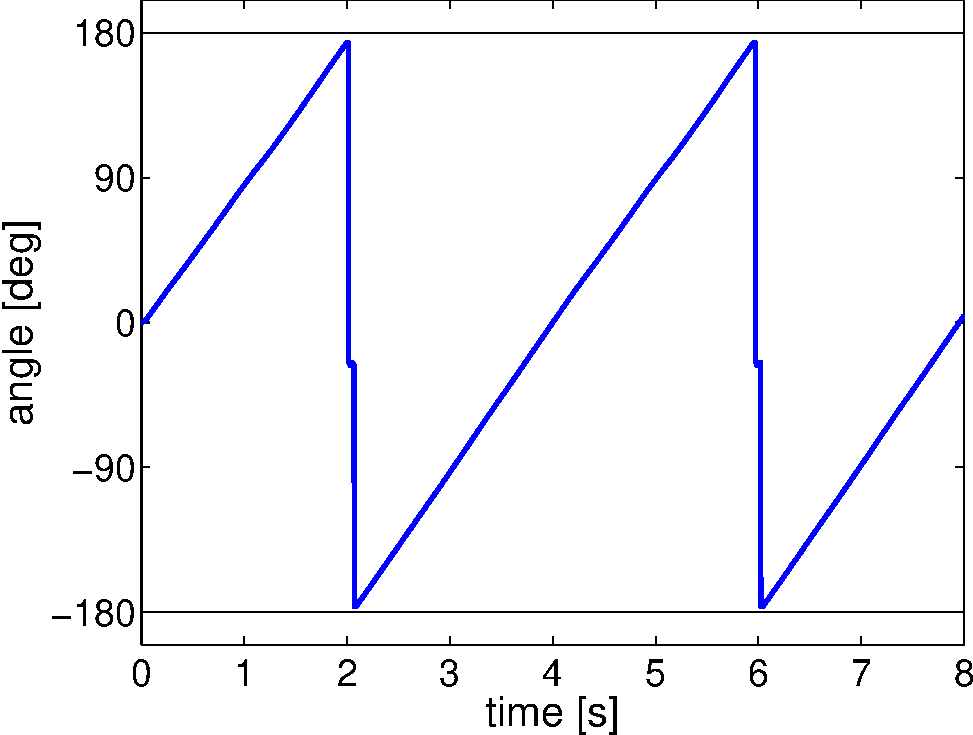
\includegraphics[scale=0.5]{sozai/figure_ad_da-crop.pdf}
  \caption{A/D,D/A変換の動作確認}
\end{figure}

\subsubsection{実験考察}
ポテンショメータには回転範囲に制限があるため,
設定された範囲(ここでは180度)に到達すると,値が再び最小値(-180度)に戻っている.
これは,ポテンショメータが無限に回転するのではなく,
ある範囲内でのみ動作するように設計されているためだと考えられている.

\subsection{P制御}

ここではアームの角度制御のためにPコントローラ
\begin{equation}
  v(t) = k_{\mathrm{P}} \left( \theta^{\text{ref}}(t) - \theta(t) \right) \quad \left( \theta^{\text{ref}}(t) : \text{目標値} , \, \theta(t) : \text{現在の角度} \right)
\end{equation}
を用い,比例ゲイン $k_{\mathrm{P}}$ を大きくするにしたがって過渡特性,定常特性がどのように変化するかを調べる.


\begin{enumerate}
  \item P制御を行うため,図3.6のSimulinkモデル“ex\_pcont.slx”を作成する.モデルはディレクトリD:\#student\_5S\#group01\#pcontに保存する.つぎに,
        \begin{verbatim}
          >> kP = 2;
        \end{verbatim}
        と入力した後,ビルドを行いエラーがないことを確認する.また,“ex\_pcont.pdf”という名前のpdfファイルを生成し,デスクトップ上の“bcpdfcrop-multi.bat”により余白を取り除く.
        
  \item ScopeとScope1を開き,リアルタイムで角度と操作量を観測できるようにする.レンズは付録A.1の図A.3に合わせる.
        
  \item センサ電圧が0 [V]となる位置にアームを動かし,“ex\_pcont.slx”を実行する.実行終了後,
        \begin{verbatim}
          >> save pcont_kP02_data t u y kP
        \end{verbatim}
        と入力し,matファイル“pcont\_kP02.data.mat”にデータを保存する.
        
        同様に,$k_{\mathrm{P}} = 4$, $k_{\mathrm{P}} = 20$と設定して“ex\_pcont.slx”を実行し,実験結果のデータを
        \begin{itemize}
          \item “pcont\_kP04.data.mat” ($k_{\mathrm{P}} = 4$)
          \item “pcont\_kP20.data.mat” ($k_{\mathrm{P}} = 20$)
        \end{itemize}
        という名前のmatファイルに保存する.
        
        最後に,配布するMファイル
        \begin{verbatim}
          >> autoplot_pcont.m
        \end{verbatim}
        を実行することによって,MATLAB上でグラフを作成する.グラフのpdfファイルは自動的に生成される.
\end{enumerate}

\subsubsection{実験結果}
以下に結果を示す.
\begin{figure}[h]
  \centering
  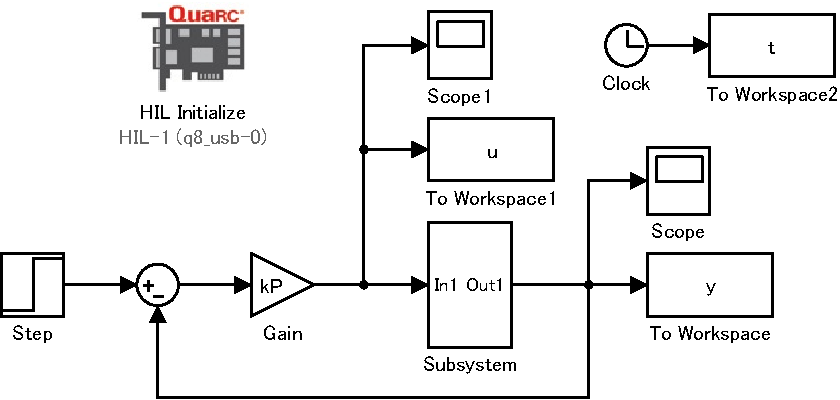
\includegraphics[scale=1]{sozai/ex_pcont-crop.pdf}
  \caption{ex\_pcont}
\end{figure}

\begin{figure}[h]
  \centering
  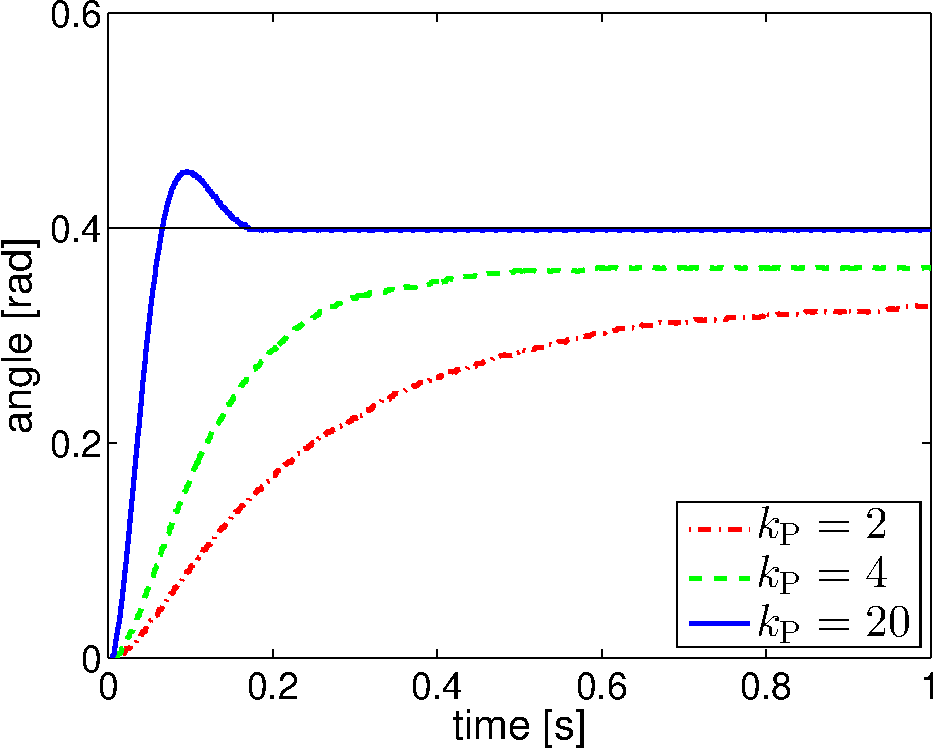
\includegraphics[scale=0.6]{sozai/figure_pcont_angle-crop.pdf}
  \caption{figure\_pcont\_angle}
\end{figure}

\begin{figure}[h]
  \centering
  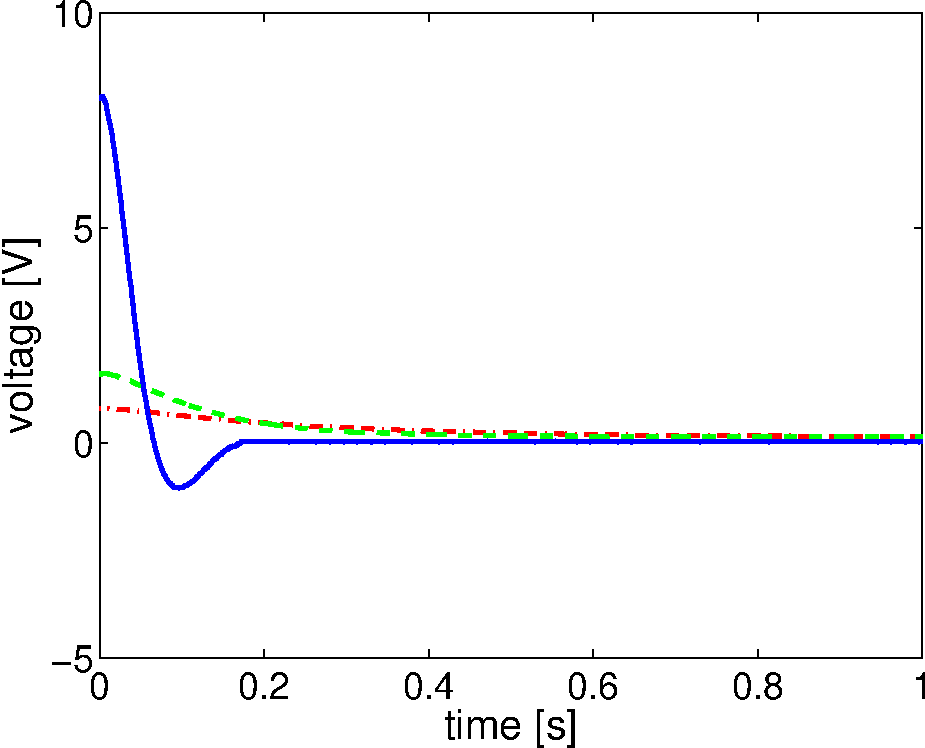
\includegraphics[scale=0.6]{sozai/figure_pcont_volt-crop.pdf}
  \caption{figure\_pcont\_volt}
\end{figure}

\subsubsection{実験考察}
図3.8と図3.9より,比例ゲイン \( k_{\mathrm{P}}\) を増加させると,
過渡特性における立ち上がり時間が短くなり,応答がより速くなることが観察できる.
これは,比例ゲイン \( k_{\mathrm{P}}\) が大きいほど制御系が目標値に迅速に追従しようとするためであり,
その結果として立ち上がり時間が短縮される.
一方で,比例ゲインが大きくなるとオーバーシュートの値も増加する傾向がある.
これは,ゲインが高いことで目標値に達する速度が増加しすぎ,目標値を超過してしまうためである.
また,操作量(入力電圧)の大きさも比例ゲイン \( k_{\mathrm{P}}\) によって増加する.
これは,制御対象が目標値から離れているときに強い制御力が働くためであり,
制御量が過大になりやすい.図3.9に示されるように, \( k_{\mathrm{P}}\) の増加に伴って初期の入力電圧が
大きくなるが,これは目標角度に迅速に追従するために必要な制御信号が大きくなるためである.
次に,定常特性(定常偏差)について考察する.比例制御のみでは,
制御対象に定常偏差が残ることがある.この理由は,比例制御が誤差に比例した制御量を出力するため,
目標値に完全に一致するためには無限大のゲインが必要となるためである.
したがって,有限の \( k_{\mathrm{P}}\)  のもとでは完全に目標値に一致することは難しい.
理論的には,最終値の定理を用いて定常偏差を考察することができる.
入力がステップ応答の場合,最終値の定理より,システムの出力 \( y(t) \) の定常値は以下で与えられる.

\begin{equation}
  \lim_{t \to \infty} y(t) = \lim_{s \to 0} s \cdot Y(s)
\end{equation}

ここで, \( Y(s) \) はシステムの出力のラプラス変換である.
比例制御のみを用いたシステムでは,定常偏差がゼロにならないため,
入力と出力の間に誤差が残る.これは,実機の摩擦や負荷変動などの外乱要因が存在するためでもある.
ポテンショメータやエンコーダのセンサー精度や摩擦力,モータの不間帯などが影響を及ぼし,
理想的な追従が難しい要因ともなっていると考えられる.


\subsection{積分動作の効果(PI制御)}

\begin{enumerate}
  \item PI 制御を行うため,図 3.7 の Simulink モデル ``ex\_picont.slx'' を作成する.モデルはディレクトリ D:\#student.5S\#group01\#picont に保存する.つぎに,
        \begin{verbatim}
        >> kP = 4; kI = 0;
    \end{verbatim}
        と入力した後,ビルドを行いエラーがないことを確認する.また,``ex\_picont.pdf'' という名前の pdf ファイルを生成し,デスクトップ上の ``bcpdfcrop-multi.bat'' により余白を取り除く.
        
  \item Scope と Scope1 を開き,リアルタイムで角度と操作量を観測できるようにする.レンズは付録 A.1 の図 A.4 に合わせる.
        
  \item センサ電圧が 0 [V] となる位置にアームを動かし,``ex\_picont.slx'' を実行する.実行終了後,
        \begin{verbatim}
        >> save picont_kP04_kI00_data t u y kP kI
    \end{verbatim}
        と入力し,mat ファイル ``picont\_kP04\_kI00.data.mat'' にデータを保存する.
        
        比例ゲインを \( k_{\mathrm{P}} = 4 \) に固定し,積分ゲインを \( k_I = 6 \),\( k_I = 12 \) として ``ex\_picont.slx'' を実行し,実験結果のデータを
        \begin{itemize}
          \item ``picont\_kP04\_kI06.data.mat'' \((k_{\mathrm{P}} = 4, k_I = 6)\)
          \item ``picont\_kP04\_kI12.data.mat'' \((k_{\mathrm{P}} = 4, k_I = 12)\)
        \end{itemize}
        という名前の mat ファイルに保存する.最後に,配布する M ファイル ``autoplot\_picont.m'' を実行することによって,MATLAB 上でグラフを作成する.グラフの pdf ファイルは自動的に生成される.
        
  \item 目標値を 0 に設定(Step の最終値を ``0'' に設定)し,また,終了時間を ``inf'' に設定する.比例ゲインを \( k_{\mathrm{P}} = 4 \) に固定し,積分ゲインを \( k_I = 0, k_I = 12 \) として実験を行い,手でアームに力を加えたとき(入力外乱を加えることに相当),反力がどうなるか調べる.
\end{enumerate}

\subsubsection{実験結果}
以下に結果を示す.
\begin{figure}[h]
  \centering
  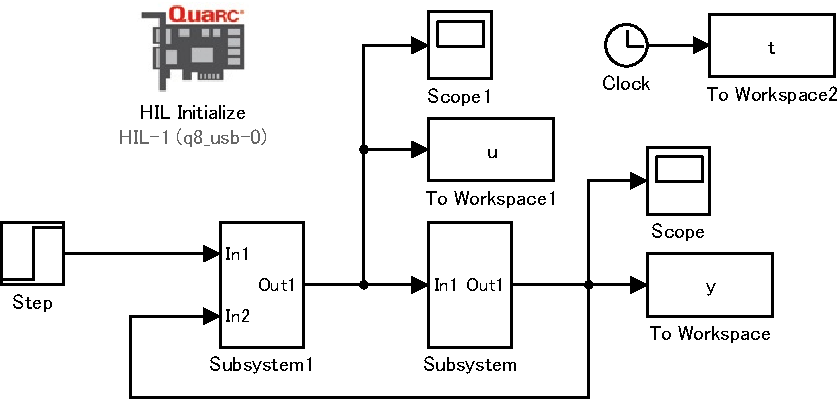
\includegraphics[scale=0.7]{sozai/ex_picont-crop.pdf}
  \caption{ex\_picont}
\end{figure}

\begin{figure}[h]
  \centering
  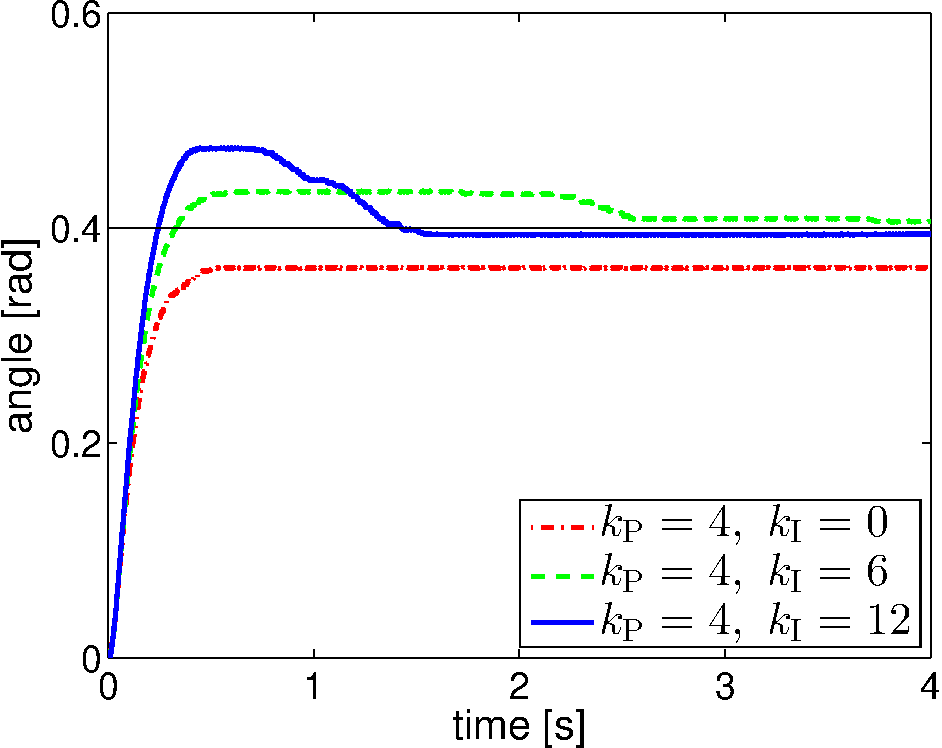
\includegraphics[scale=0.5]{sozai/figure_picont_angle-crop.pdf}
  \caption{figure\_picont\_angle}
\end{figure}

\begin{figure}[h]
  \centering
  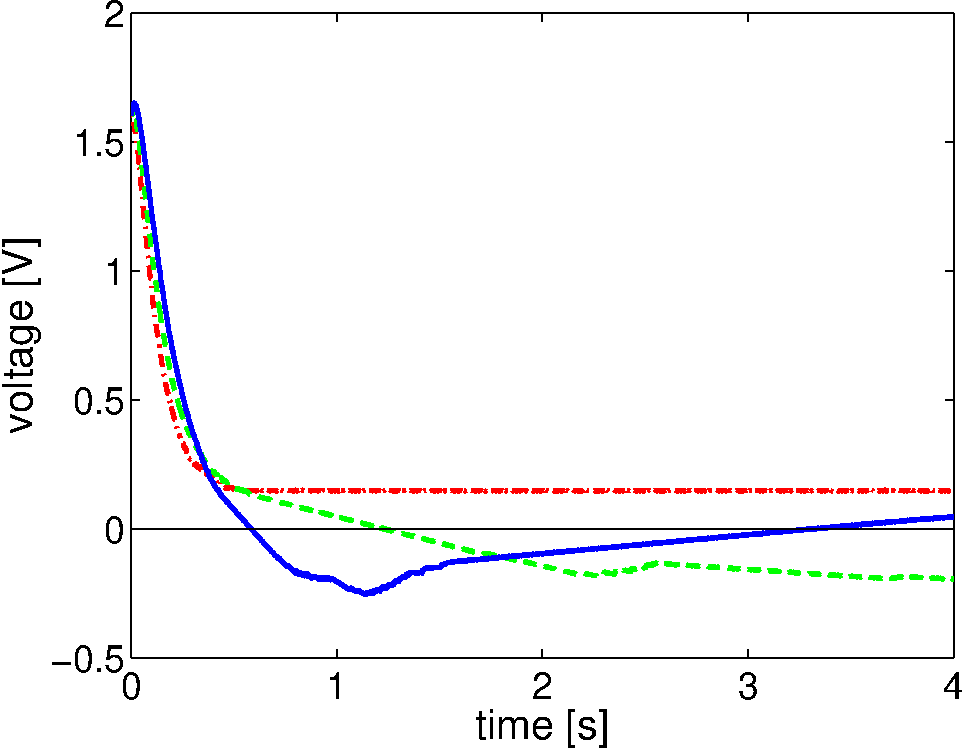
\includegraphics[scale=0.5]{sozai/figure_picont_volt-crop.pdf}
  \caption{figure\_picont\_volt}
\end{figure}

\newpage

\subsubsection{実験考察}
積分動作の導入により,定常偏差が収束したことが図3.11よりわかる.
定常偏差が収束した理由は,積分動作が偏差の累積に基づいて補正を行うためである.
制御系において,積分動作は偏差が存在する限り制御信号を加え続け,目標値に到達するまでその効果を増大させる.
これにより,定常偏差が時間とともに蓄積されて制御信号として反映され,
結果として定常偏差が収束する形で解消されるため,最終的にシステムは目標値に到達する.
さらに,アームに外力が加わった場合,P制御の場合,差分におおじた出力のみであったが,
PI制御の場合,偏差が蓄積され,徐々に出力が大きくなる.


